% Originally: LuxSleek-CV 1.1 LaTeX template
% Original Author: Andreï V. Kostyrka, University of Luxembourg
% Moderately Modified by Ali Abdou for content, design, and visuals

\documentclass[12pt, a4paper]{article} 

\usepackage[T1]{fontenc}
\usepackage[utf8]{inputenc}  
\usepackage[british]{babel}  
\usepackage[left = 0mm, right = 0mm, top = 0mm, bottom = 0mm]{geometry}
%\usepackage[stretch = 25, shrink = 25, tracking=true, letterspace=30]{microtype}  
\usepackage{graphicx}        
\usepackage{xcolor}          
\usepackage{marvosym}        
\usepackage{enumitem}      
\usepackage{tikz}
%\setlist{parsep = 0pt, topsep = 0pt, partopsep = 1pt, itemsep = 1pt, leftmargin = 3em}


\usepackage[default,oldstyle,scale=0.95]{opensans}

\usepackage{fontawesome5}

\definecolor{cvblue}{HTML}{164194}

%%%%%%% COMMAND DEFINITIONS %%%%%%%%%%%%%%%%%%%%%%%%%%%
\newcommand{\dates}[1]{\hfill\textsc{\footnotesize\color{cvblue}#1}} 
\newcommand{\location}[1]{\hfill\textsc{\footnotesize{#1}}}
\newcommand{\jobtitle}[1]{\textbf{#1}} 
\newcommand{\is}{\vspace{1.6ex}\vskip.5ex plus .4ex} 
\newcommand{\smaller}[1]{{\small$\bullet$\ #1}}
\newcommand{\headleft}[1]{\vspace*{3ex}\textsc{\textbf{#1}}\par%
    \vspace*{-1.5ex}\hrulefill\par\vspace*{0.7ex}}
\newcommand{\headright}[1]{\vspace*{2.5ex}\textsc{\Large\color{cvblue}#1}\par%
     \vspace*{-2ex}{\color{cvblue}\hrulefill}\par}
%%%%%%%%%%%%%%%%%%%%%%%%%%%%%%%%%%%%%%%%%%%%%%%%%%%%%%%%%%%%

\usepackage[colorlinks = true, urlcolor = white, linkcolor = white]{hyperref}

\begin{document}

\setlength{\topskip}{0pt}
\setlength{\parindent}{0pt}
\setlength{\parskip}{0pt}
\setlength{\fboxsep}{0pt}
\pagestyle{empty}
\raggedbottom

\begin{minipage}[t]{0.33\textwidth} 
\colorbox{cvblue}{\begin{minipage}[t][6mm][t]{\textwidth}\null\hfill\null\end{minipage}}

\vspace{-.2ex}
\colorbox{cvblue!85}{\color{white}  
\kern0.09\textwidth\relax
\begin{minipage}[t][293mm][t]{0.82\textwidth}
\raggedright
\vspace*{2.5ex}

\null\hfill\begin{tikzpicture}
    \clip (0,0) circle(2.1cm);
    \node at (0,0){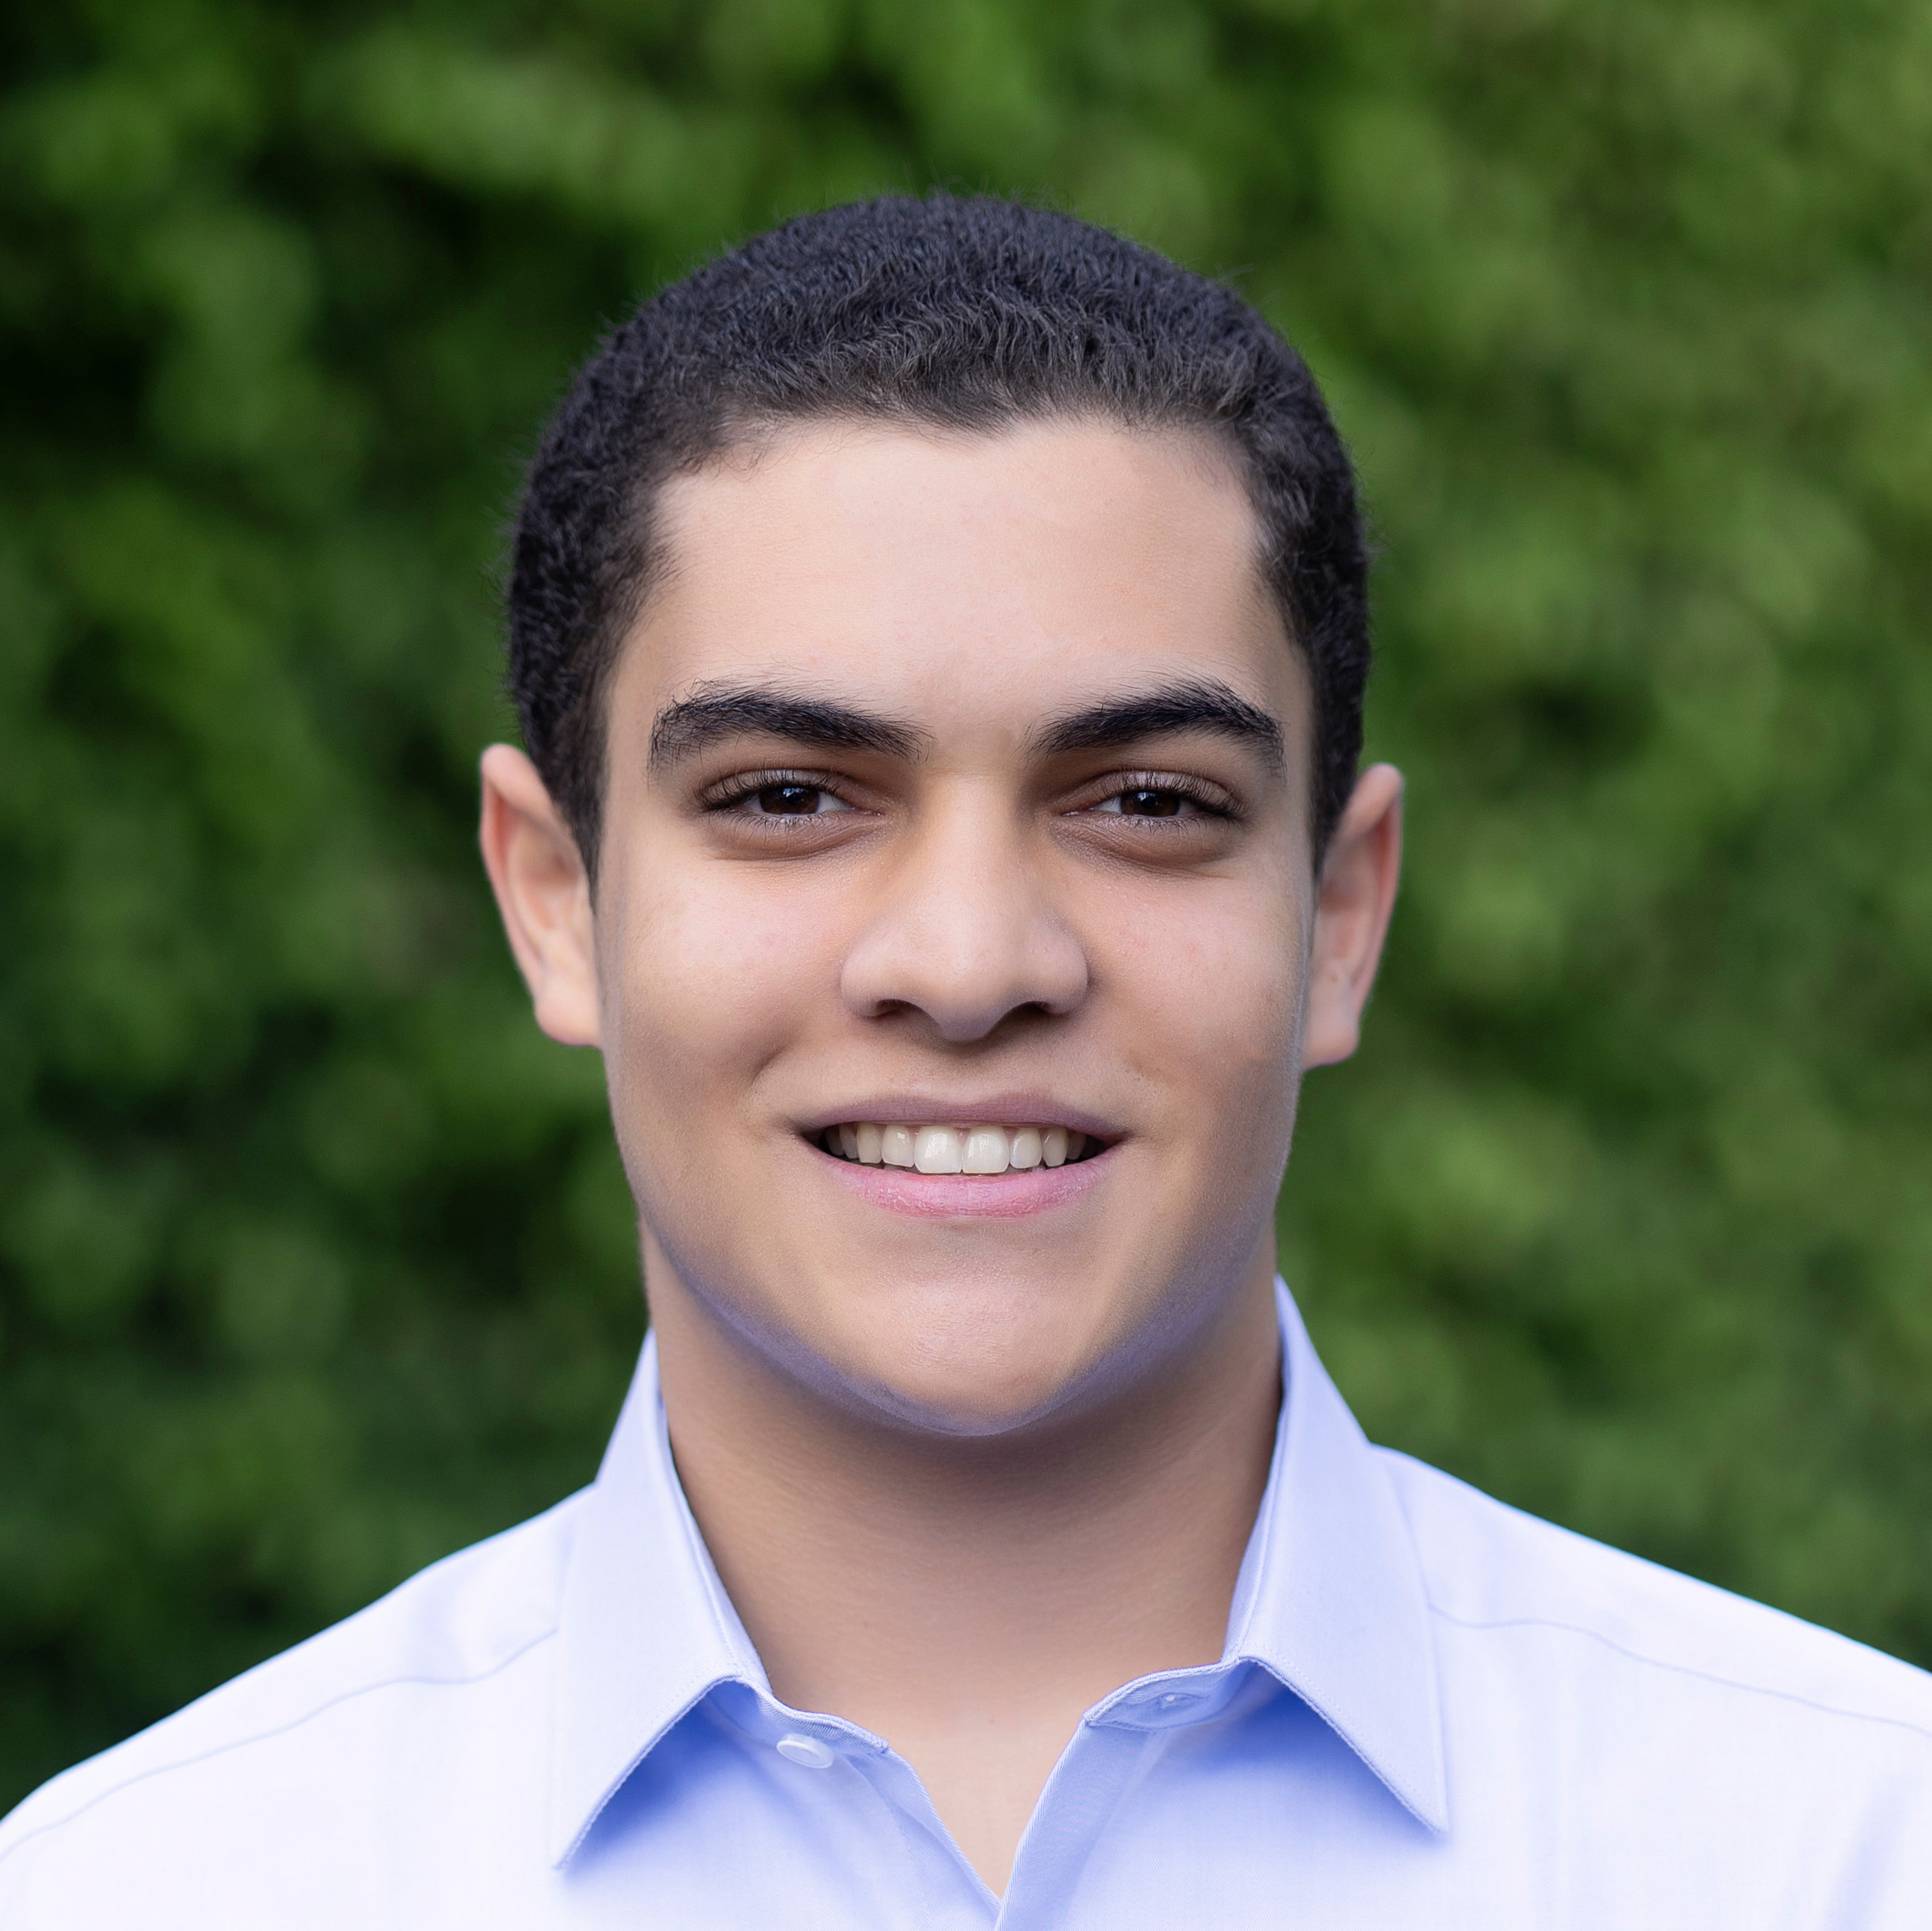
\includegraphics[width=4.8cm,height=4.8cm]{../images/me.png}};
\end{tikzpicture}\hfill\null

\vspace*{1.7ex}

\centering{\Large\textbf{\textsc{Ali Abdou}}}\par\raggedright \normalsize 

\vspace*{0.5ex} 

\headleft{About Me}
BSc Computer Science student at Gisma University of Applied Sciences in Berlin, Germany. Passionate about technology, leadership, and innovation. Founder of \textbf{ENMUN}, aiming to connect youth with change-making. Currently completing Harvard CS50 and TU Delft math courses.

\headleft{Contact Details}
\small
\begin{tabular}{@{}l@{\hspace{1em}}l@{}}
    \faLink & www.aliabdou.de \\[0.5ex]
    \Letter & me@aliabdou.de \\[0.5ex]
    \faMobile & +49\, 152\, 25379483 \\[0.5ex]
    \faLinkedin & \href{https://linkedin.com/in/aliabdouu}{in/aliabdouu}
\end{tabular}

\normalsize

\headleft{Languages}
\begin{tabular}{@{}l@{\hspace{1em}}l@{}}
    \textbf{Arabic} & Native \\[0.5ex]
    \textbf{English} & C2 \\[0.5ex]
    \textbf{German} & A2 \\[0.5ex]
\end{tabular}

\headleft{Certifications}
\begin{itemize}[leftmargin=0.7em, label={$\bullet$}, topsep=0pt, partopsep=0pt, parsep=0pt, itemsep=4pt]
        \item {RedBull On-Premise Sales Simulation (Forage, May 2023)}
        \item {Advanced Python Programming (Nile University, Aug 2019)}
        \item {Introduction to Web Design (HTML, CSS, JS) (Nile University, Aug 2017)}
        \item {Introduction to Python Programming (Nile University, Aug 2015)}
\end{itemize}

\end{minipage}%
\kern0.09\textwidth\relax
}
\end{minipage}%
\hskip2.5em
\begin{minipage}[t]{0.56\textwidth}
\setlength{\parskip}{0.8ex}

\vspace{2ex}

\headright{Experience}

\jobtitle{IT Infrastructure Intern}  \location{Cairo, Egypt} \\
\textsc{Orascom Development}  \dates{Aug 2023} \\
\smaller{Installed wireless access points and VoIP lines in OHD’s new office} \\
\smaller{Maintained wireless access points and VoIP lines in OHD’s main office} \\
\smaller{Troubleshooted Microsoft Azure policy conflicts \& set up new-hire devices} 

\is
\jobtitle{Sales \& Marketing Intern}  \location{Cairo, Egypt} \\
\textsc{Rizme}  \dates{Nov 2022--Mar 2023} \\
\small{Conducted competitor analysis and reached out to clients during the development of multiple projects. Testing brand new “Closeara” property management app on iOS devices. Brainstormed features for clients such as the youth startup “Toot” and the newly-launched "G.Ride" by MATGR.}

\is
\jobtitle{Student Ambassador}  \location{Remote} \\
\textsc{Lapse}  \dates{Jul--Sep 2022} \\
\small{Represented and tested a new invite-only app known as Journal. Journal is a form of disposable camera designed to stop people from craving likes/comments and instead living in the moment and forgetting about filters and edits.}

\headright{Education}

\jobtitle{Gisma University of Applied Sciences}  \location{Berlin, Germany}\\
\normalsize{Computer Science, Bachelor of Science} \dates{Oct 2024--Present}\\
\small{180 ECTS programme, EQF Lvl 6} 

\is
\jobtitle{American International School in Egypt -- West }  \location{Cairo, Egypt}\\
\normalsize{International Baccalaureate Diploma} \dates{Sep 2010--June 2024}\\
\small{Higher Levels:
    \begin{itemize}[leftmargin=3em, label={$\bullet$}, topsep=0pt, partopsep=0pt, parsep=0pt, itemsep=0pt]
        \item {Computer Science}
        \item {Physics}
        \item {Mathematics Analysis \& Approaches}
    \end{itemize}
}
\small{Standard Levels:
    \begin{itemize}[leftmargin=3em, label={$\bullet$}, topsep=0pt, partopsep=0pt, parsep=0pt, itemsep=0pt]
        \item {English A: Language \& Literature}
        \item {French ab initio}
        \item {Business Management}
    \end{itemize}
}
\small{Core:
    \begin{itemize}[leftmargin=3em, label={$\bullet$}, topsep=0pt, partopsep=0pt, parsep=0pt, itemsep=0pt]
        \item {Theory of Knowledge}
        \item {Extended Essay in Business Management}
    \end{itemize}
} 

\is
\jobtitle{Zewail City of Science and Technology} \location{Cairo, Egypt} \\
\normalsize{Summer Program}   \dates{Aug 2022} \\
\small{Courses:
    \begin{itemize}[leftmargin=3em, label={$\bullet$}, topsep=0pt, partopsep=0pt, parsep=0pt, itemsep=0pt]
        \item {Environmental Sciences}
        \item {Mathematics}
        \item {Physics}
        \item {Biology}
        \item {Robotics}
        \item {Renewable Energy Engineering}
    \end{itemize}
}

\end{minipage}
\end{document}
